\section{HDAC6 Structure and Function}

One such host protein with the potential to be a drug target is histone deacetylase 6 (HDAC6), along with the molecular motors myosin 10 and dynein, and their respective cytoskeletal filaments \cite{banerjee2014influenza}.

Histone deacetylases are a class of enzymes that remove acetyl groups from chromatin and other acetylated proteins. Currently 18 HDAC proteins are known, which are classified into 4 classes. HDAC6 belongs to the IIb class, which is primarily localized in the cytoplasm \cite{hai2016histone}.

Among other histone deacetylases, HDAC6 is the only one to carry tandem catalytic domains CD1 and CD2 (Figure \ref{figure:HDAC6Domains}). The dynein motor binding (DMB) domain is located between them. HDAC6 also has a ubiquitin-binding domain ZnF ("zinc-finger") which senses polyubiquitinated misfolded protein cargo \cite{hai2016histone}. HDAC6-ZnF selectively binds \cite{zhang2008mice} to ubiquitin chains with unanchored C-terminal diglycine \cite{ouyang2012protein}.

\begin{figure}
\begin{center}
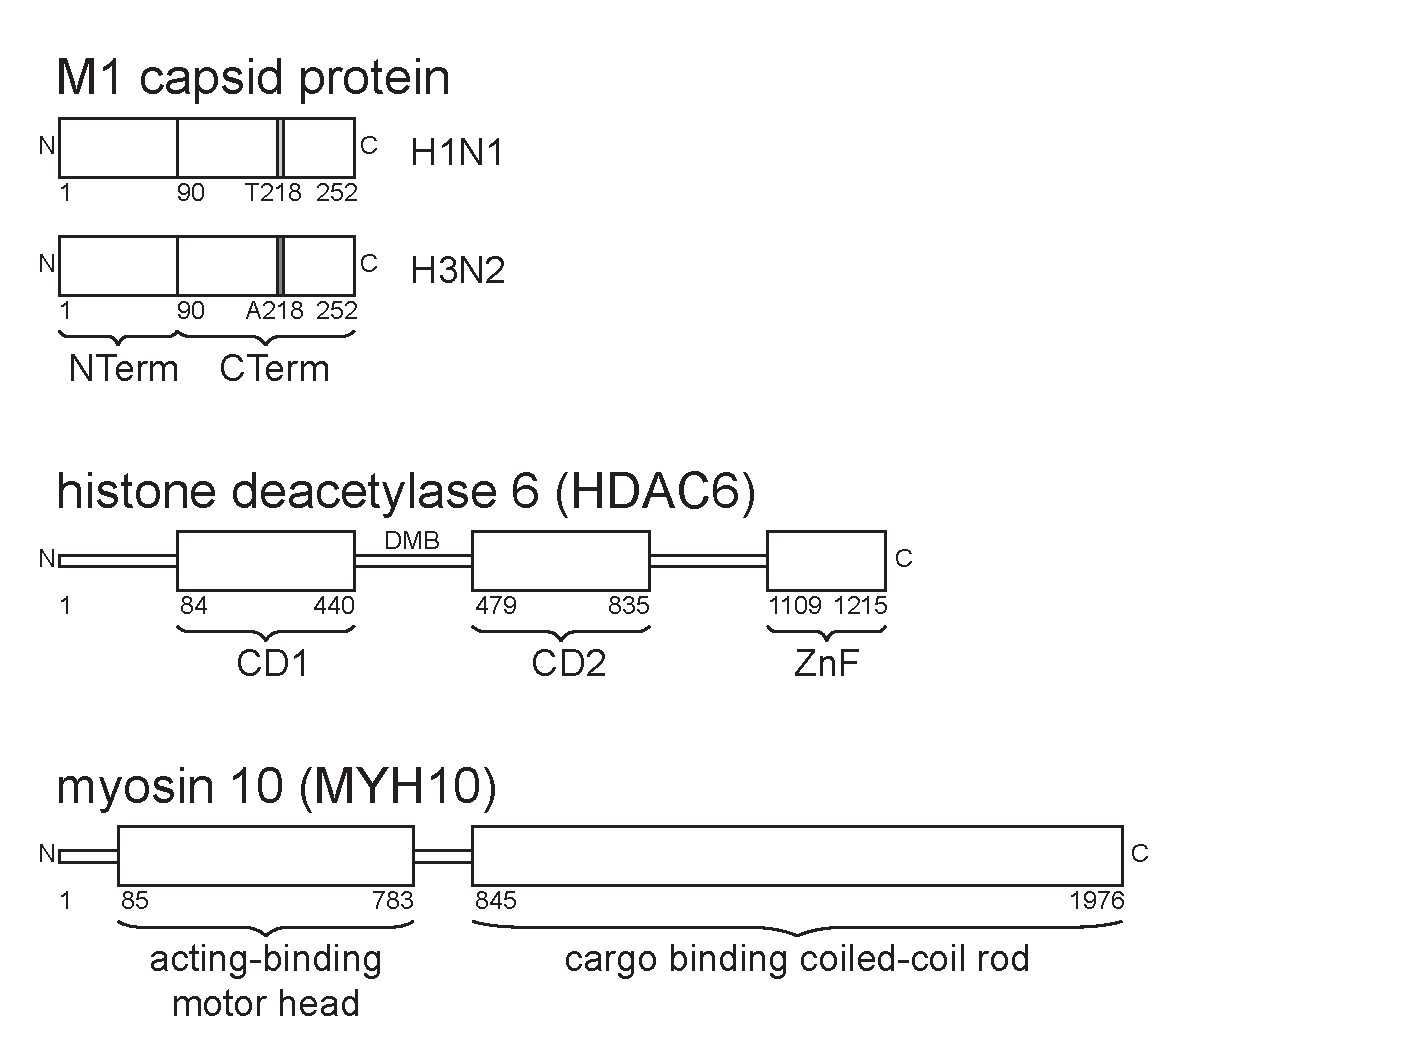
\includegraphics[width=1\textwidth, trim={0cm 6cm 8cm 8.8cm}, clip]{D_chapters/0_introduction/protein_domains.pdf}
\caption[HDAC6 domain organization]{HDAC6 domain organization \par
CD1 and CD2 - catalytic domains, DMB - dynein motor binding domain, ZnF - ubiquitin binding domain "zinc-finger". N and C denote N- and C-terminus. Numbers denote amino acid residues.}
\label{figure:HDAC6Domains}
\end{center}
\end{figure}

HDAC6 deacetylates tubulin \cite{zhang2003hdac, zhang2008mice} (polymer making up the microtubules), and heat shock protein 90 (Hsp90) \cite{kovacs2005hdac6} (a chaperone protein which assists protein folding and degradation). HDAC6 senses ubiquitinated protein aggregates and triggers their clearance \cite{boyault2007hdac6}. HCAC6 also assists in stress granule formation and cellular oxidative stress recovery \cite{kwon2007deacetylase}.

During influenza infection, HDAC6 (specifically, HDAC6-ZnF) and other components of the aggresome processing machinery - molecular motors myosin 10 and dynein - were essential for efficient uncoating. Involvement of molecular motors suggested that influenza uncoating is achieved through physical forces generated by microtubule- and actin-associated motors \cite{banerjee2014influenza}.

\section{Open questions in influenza uncoating}

Uncoating is a limiting step in influenza infection \cite{banerjee2013high}. Previously, influenza uncoating has been described as a passive process, relying on pH-controlled fusion pore formation and conformation changes in M1 capsid proteins \cite{zhang2012dissection}. Recruitment of HDAC6 and molecular motors in uncoating \cite{banerjee2014influenza} highlights that it is instead an active process which involves cellular proteins.

Molecular motors may regulate viral genome localization after uncoating \cite{qin2019real} by assisting viral transport to correct cellular compartments. This is commonly described through tug-of-war mechanism, which involves velocity and force balance between all involved parties. It has been previously suggested as a process controlling cellular cargo and viral transport \cite{gazzola2009stochastic}. Modelling studies focus on tug-of-war between two types of microtubule motors with opposing processivity \cite{muller2008tug, gazzola2009stochastic}.

Others suggest that during viral infection tug-of-war between microtubule molecular motors may act as a force generating mechanism instead \cite{strunze2011kinesin,lukic2014hiv}. Involvement of myosin 10 and dynein in both endosomal and acid bypass uncoating during influenza infection is consistent with a force generation thorugh tug-of-war between different types of molecular motors: actin filament and microtubule ones. Whether such a mechanism exist, and is able to generate enough force to break influenza capsid is unclear.

Another intriguing aspect is the role of ubiquitin (Ub) in influenza viral uncoating. Influenza virus particles carry significant amounts of cellular Ub B \cite{hutchinson2014conserved}. Ubiquitination assists viral uncoating \cite{rudnicka2016ubiquitin}. HDAC6-ZnF deletion leads to reduction of influenza uncoating \cite{banerjee2014influenza}, indicating Ub involvement in the process. One possibility is that viral Ub serves as an interface between viral capsid protein M1 and HDAC6, competing with cellular Ub. Alternatively, Ub may instead assist motor recruitment, in which case viral Ub may only provide advantage in localization, but otherwise would serve the same function as cellular Ub. These possibilities would also impact interfaces between HDAC6 and molecular motors. HDAC6 is known to bind dynein through its DMB domain \cite{kawaguchi2003deacetylase}. The exact mechanism or location of myosin interaction with HDAC6 is unclear.
